%&LaTeX
% !TEX encoding = UTF-8 Unicode
\documentclass{article}
\usepackage[utf8]{inputenc}
\usepackage[francais]{babel}
\usepackage[T1]{fontenc}
\usepackage{textcomp}
\usepackage[colorlinks=true, linkcolor=black, urlcolor = blue]{hyperref}

\usepackage{graphicx}
\usepackage{ulem}
\usepackage{color}
\usepackage[top=2cm,bottom=2cm,left=2.5cm,right=2.5cm]{geometry}

\definecolor{color01}{rgb}{0.00,0.00,0.00}
\definecolor{color02}{rgb}{0.40,0.40,0.40}
\definecolor{color04}{rgb}{0.07,0.33,0.80}
\definecolor{color05}{rgb}{1.00,0.00,0.00}


\title{\Huge{AGETAC\\
Aide à la GEstion TACtique\\}
\huge{{\color{color02} \textit{Manuel d'utilisation}}}}

\date{Mai 2012}
\author{Projet Agetac - Université de Rennes 1\\
Encadré par Noël Plouzeau}



\begin{document}
\maketitle
\vspace{1.1in}
\tableofcontents
\newpage
 \section{Objectifs}

Faciliter la gestion d'une intervention. Les tablettes inter-connectées 
au serveur apporteront plus de rapidité et de précision, améliorant ainsi le 
bon déroulement d'une intervention.

\section{Utilisation de la tablette}

Toujours s'assurer que la tablette dispose de suffisamment de 
batterie. Celle-ci doit pouvoir rester en marche pendant toute la durée d'une 
intervention.

\subsection{Connexion à une intervention}

Avant de se rendre sur les lieux du sinistre, ou une fois sur 
place, mettre la tablette sous tension et s'identifier.

Une fois la connexion établie, l'onglet SITAC apparaît à l'écran. 
Il s'agit de l'onglet d'accueil.

Vous pouvez ensuite naviguer entre les différents onglets d'une 
simple pression sur ceux-ci.

\subsection{Présentation des différents onglets}

\subsubsection{Onglet SITAC}

Cet onglet permet de visualiser l'intervention.

Il est composé d'une carte et d'un menu d'outils sur la gauche. 
Celui-ci permet de représenter le sinistre grâce aux différents pictogrammes 
regroupés dans le menu d'outils.

\begin{figure}[htbp]
\begin{center}
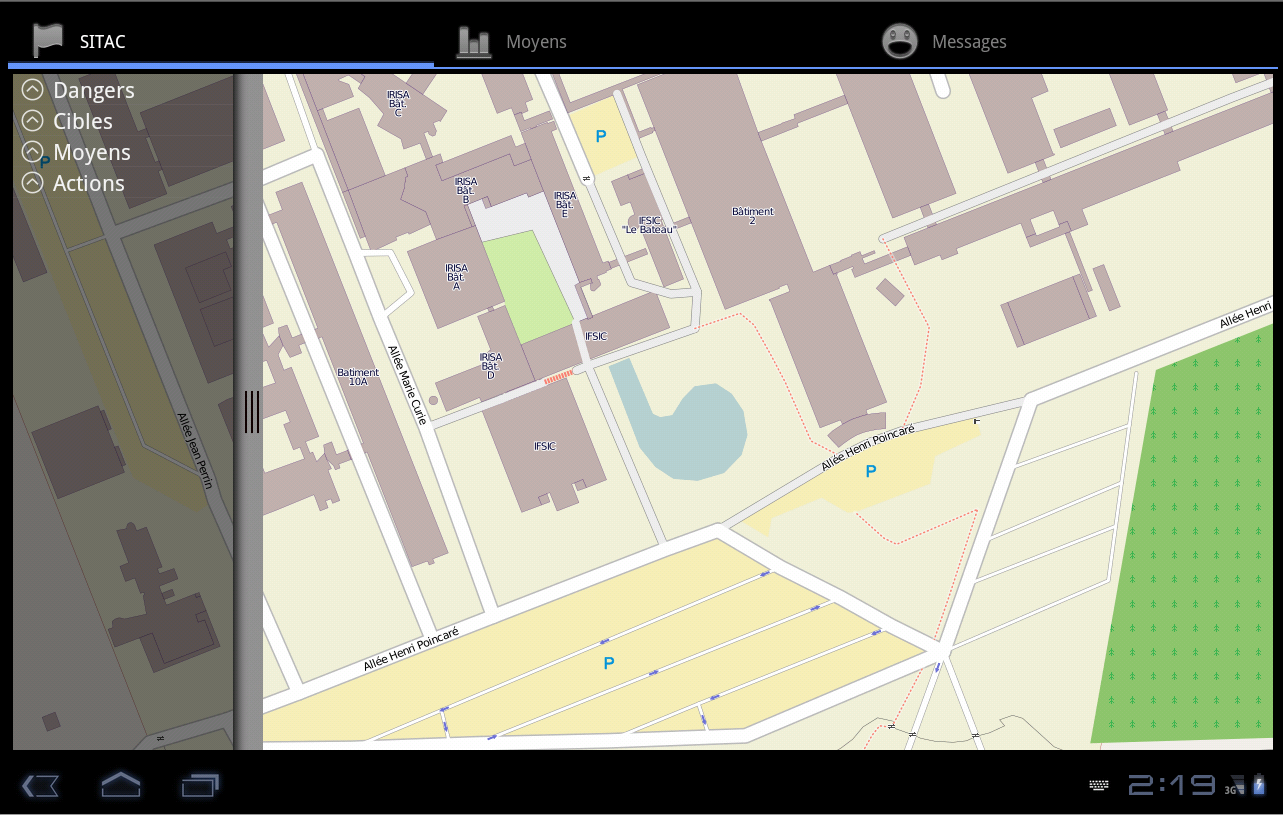
\includegraphics[width=487pt, height=309pt]{Manueldutilisation-fig001.png}
\caption{Vue de la SITAC}
\end{center}
\end{figure}

\subsubsection{Onglet Moyens}

Cet onglet référence les moyens demandés et présents sur les 
lieux. Il permet de faire des demandes qui seront automatiquement transmises au 
CODIS, ou de renvoyer un véhicule si sa présence n'est plus nécessaire à l'intervention. 
On peut aussi y consulter tout ce qui est relatif à chaque véhicule (sa 
caserne d'origine, son groupe horaire de demande, d'arrivée, 
de départ)

\begin{figure}[htbp]
\begin{center}
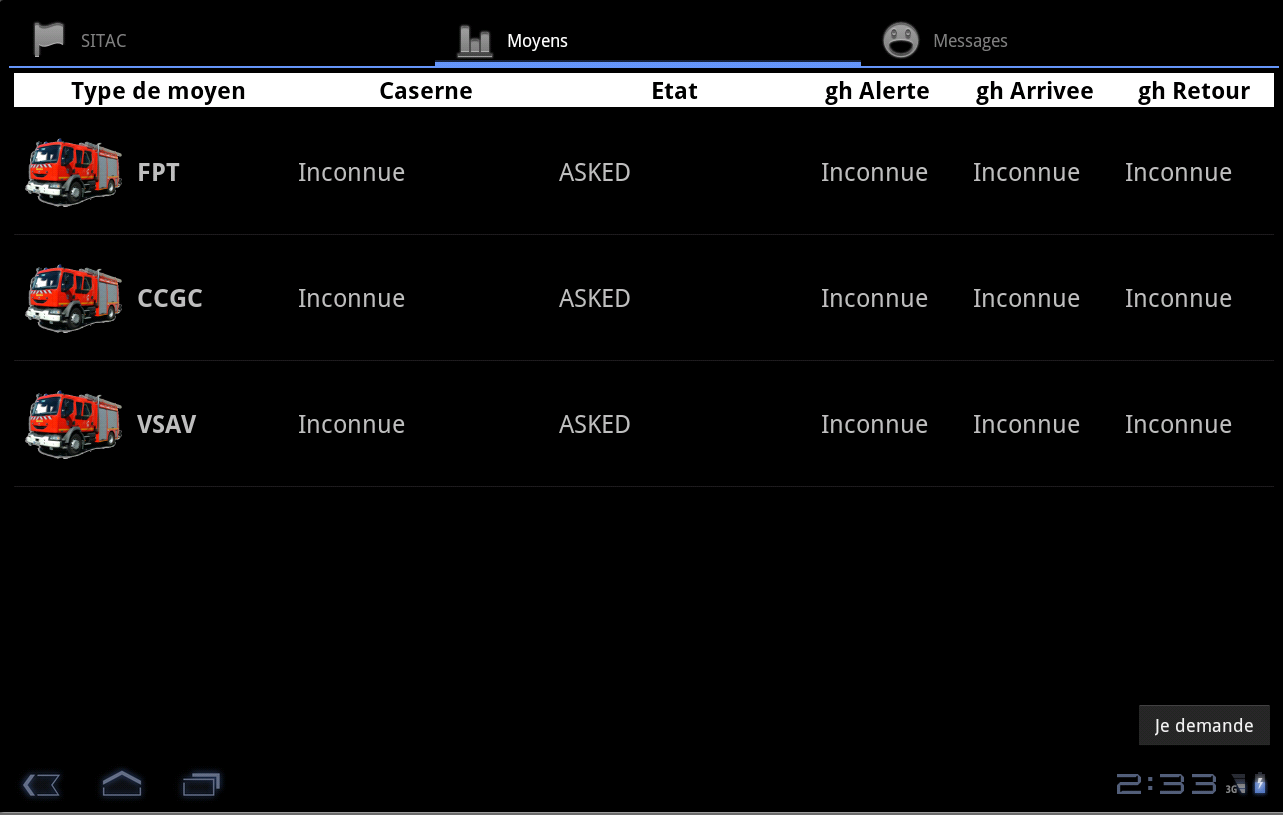
\includegraphics[width=487pt, height=309pt]{Manueldutilisation-fig002.png}
\caption{Tableau des moyens}
\end{center}
\end{figure}


\subsubsection{Onglet Messages}

Cet onglet permet d'envoyer des messages au CODIS, ou de consulter 
l'historique des messages envoyés tout au long de l'intervention en cours.

\begin{figure}[htbp]
\begin{center}
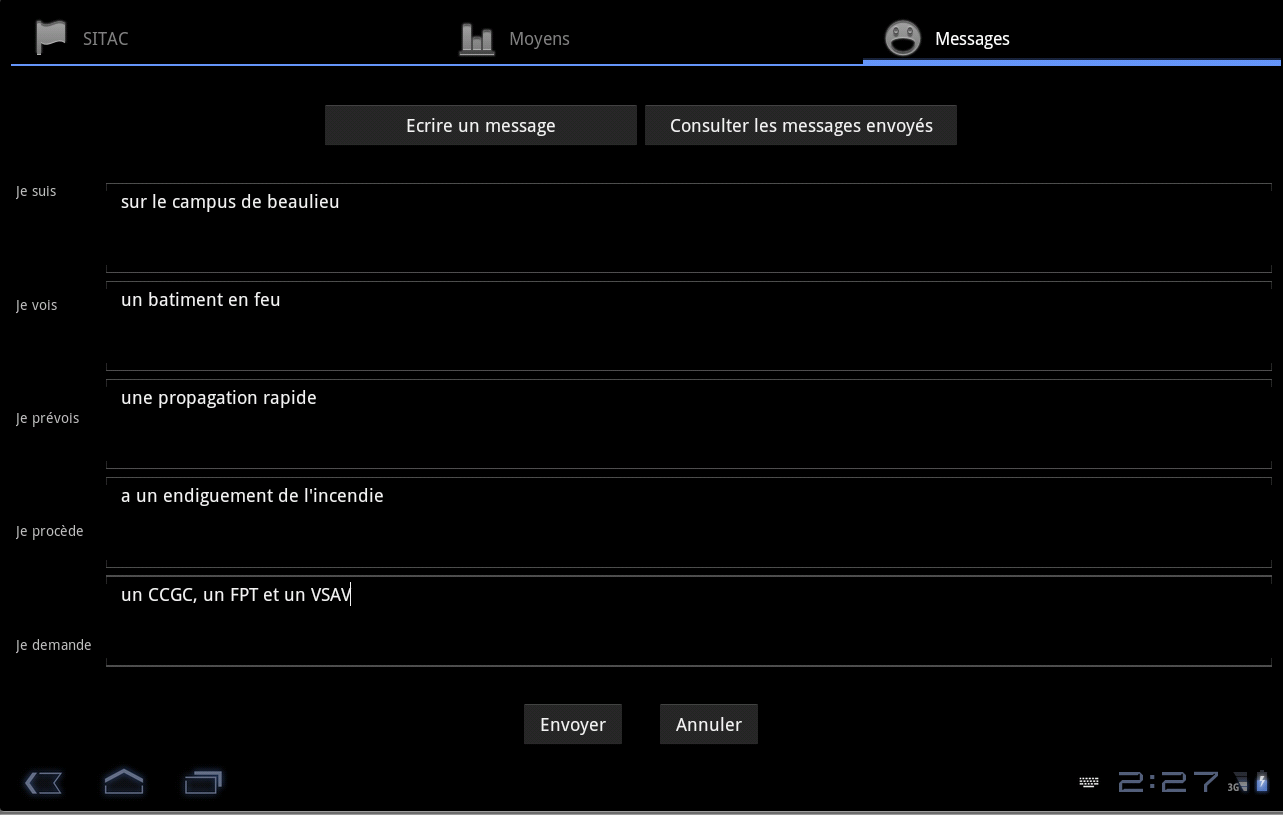
\includegraphics[width=487pt, height=309pt]{Manueldutilisation-fig003.png}
\caption{Vue message d'ambiance}
\end{center}
\end{figure}

\begin{figure}[htbp]
\begin{center}
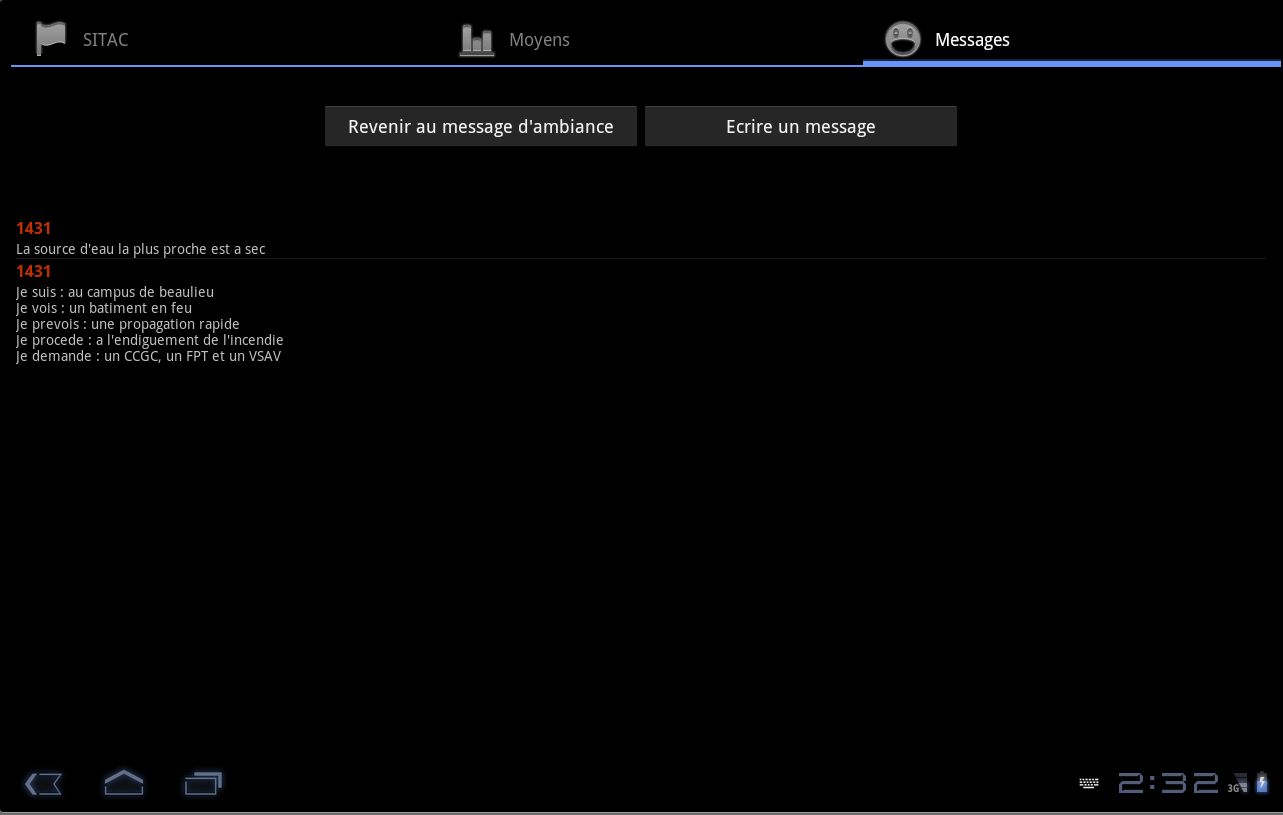
\includegraphics[width=487pt, height=309pt]{Manueldutilisation-fig004.png}
\caption{Historique des messages envoyés}
\end{center}
\end{figure}

\subsection{Manipuler la SITAC}


\subsubsection{Zoom}

Grâce à la géolocalisation, la carte se charge automatiquement 
en fonction de votre position.

Vous pouvez zoomer ou dézoomer celle-ci en effleurant les boutons 
zoom/dézoom situés en bas de l'onglet.


\subsubsection{Placer des pictogrammes}

Pour ajouter des éléments à la carte, déroulez le menu de 
gauche, les outils y sont classés par catégorie, sélectionnez une catégorie 
puis l'élément voulu et placez-le sur la carte à l'endroit désiré.


\subsubsection{Délimiter une zone sur la carte}

Choisir l'outil ``ligne'' puis le placer sur la carte de manière 
à encercler la zone, tout en s'assurant que les extrémités des lignes soient 
en contact.


\subsubsection{Demander un moyen depuis la SITAC}

Sélectionnez le véhicule voulu dans le menu de gauche, et positionnez-le 
sur la carte à l'endroit ou celui-ci devra stationner à son arrivée sur les 
lieux du sinistre. Cette action déclenchera systématiquement la demande de ce 
véhicule auprès du centre de secours le plus proche.

Pour annuler une demande de moyen, appuyez quelques secondes sur 
le véhicule que vous venez de rajouter sur la carte puis cliquez sur la croix 
qui apparaît.


\subsection{Faire une demande de moyen}

Il est possible de faire une demande de moyen via l'onglet moyen 
ou en plaçant directement un véhicule sur la SITAC.

Depuis l'onglet moyen, cliquer sur le bouton ``Je demande''situé 
en bas à droite de l'écran, un menu pop-up apparaîtra, sélectionner ensuite 
la catégorie du véhicule voulu puis dans la liste de véhicule sélectionner 
un véhicule. Une demande de ce moyen sera immédiatement transmise.

Tout véhicule demandé se retrouvera dans la liste des véhicules 
ainsi que leur état (demandé, arrivé, rentré).

Des camions appraissent sans qu'on les demandent dans l'onglet 
des moyens, et quand on clique dessus et que l'on fait supprimer, l'appli plante 
et on a un nullPointerExpection.


\subsection{Gestion des moyens }

La gestion des moyens se fait depuis l'onglet ``Moyens'' Vous 
pouvez a tout moment consulter les véhicules impliqués dans l'intervention, ainsi 
que toutes les informations les concernant.

La vue d'accueil se présente sous la forme d'un tableau regroupant 
les détails concernant les moyens engagés c'est à dire le type du moyen, sa 
provenance, son état (demande, arrivé, rentré), et les groupes horaires d'alerte, 
d'arrivée et de retour.

Pour effectuer des modifications sur l'un des véhicules présent 
dans le tableau, faire un appui long sur celui-ci et d'éditer les informations 
choisies.


\subsection{Envoyer/Consulter des messages}

Dans l'onglet message, il est possible d'envoyer des messages, 
ou de consulter un historique des messages envoyés.

Concernant l'envoi, il existe deux types de messages, message 
d'ambiance, ou message standard.

\begin{itemize}
\item Pour un message d'ambiance : complétez les champs ``je suis 
/ je vois / je prévois / je procède / je demande'' puis appuyez sur le bouton 
envoyer.

\item Pour un message standard : tapez le message voulu dans la zone 
de texte puis appuyez sur le bouton envoyer.
\end{itemize}

Vous pouvez annuler votre saisie à l'aide du bouton ``Annuler''qui 
videra tous les champs de saisie.

Concernant la consultation de l'historique des messages envoyés, 
il suffit d'appuyer sur le bouton ``consulter les messages envoyés''et s'affiche 
alors à l'écran la liste de tous les messages que vous avez envoyé depuis le 
début de l'intervention. Celui envoyé le plus récemment étant en tête de liste. 


Pour naviguer entre les différentes sous-catégories de l'onglet 
message, il vous suffit d'utiliser les boutons situés en haut de page, qui vous 
permettront de passer du message standard aux messages d'ambiance ou aux messages 
envoyés.  Ces boutons sont toujours présents en haut de page sur les différentes 
vues.

\end{document}
